\chapter{Testy systemu sterującego}
\label{cha:testy}

W tym rozdziale zostały omówione badania sieci neuronowej. Ich głównym celem jest sprawdzenie poprawności jej działania, określenie optymalnej topologii sieci oraz układu połączeń między neuronami.

\section{Testy poprawności działania sztucznej sieci neuronowej}

Ze względu na nietrywialną implementację zagadnień związanych z sieciami neuronowymi oraz algorytmów uczących, sieć została przetestowana pod kątem poprawności działania na zdecydowanie prostszym zagadnieniu jakim jest operacja logiczna typu XOR.

Została ona wybrana ze względu na łatwość zrozumienia problemu, bezproblemowe określenie oczekiwanego wyniku oraz brak wymaganego zbioru uczącego - wektor wejściowy może on zostać wygenerowany podczas samego procesu uczenia, natomiast wartość oczekiwana zostaje obliczona przy pomocy prostej operacji logicznej.

\begin{table}
\centering
\label{tab:expected_xor_output}
\begin{tabular}{|r|l|l|}
  \hline 
  Wejście 1 & Wejście 2 & Wyjście \\
  \hline 
  0 & 0 & 0 \\
  \hline
  0 & 1 & 1 \\
  \hline
  1 & 0 & 1 \\
  \hline
  1 & 1 & 0 \\
  \hline
\end{tabular}
\caption{Oczekiwane wartości odpowiedzi sieci realizującej xor.}
\end{table}

Na podstawie \ref{tab:expected_xor_output} łatwo zauważyć, iż operacja te jest nieliniowa. Cecha ta powoduje, iż pojedyńczy do realizacji tego problemu wymagana jest sieć wielowarstwowa - z przynajmniej jedną warstwą ukrytą. Do rozwiązania tego zagadnienia zastosowano dipolarną funkcję sigmoidalną - tangens hiperboliczny.
Działanie sieci neuronowej zostało sprawdzone w dwuch przypadkach. Pierwszy z nich dla niewystarczającej ilości neuronów potrzebnych do realizacji tego zagadnienia. Następnie drugi przypadek wykorzystuje odpowiednią architekturę sieci potrzebną do realizacji zagadnienia, aby wykazać poprawność działania implementacji.

\begin{figure}[!htbp]
\centering
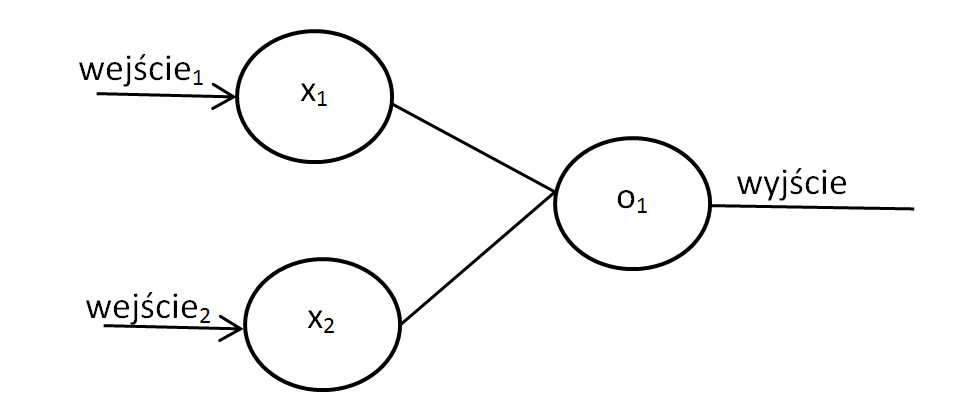
\includegraphics[width=0.7\linewidth]{./include/flow_2_1}
\caption{Przepływ informacji w topologii 2-1.}
\label{fig:flow_2_1}
\end{figure}

Na wykresie \ref{fig:neuro_2_1} przedstawiono proces uczenia sieci. Zawiera on informacje o błędach odpowiedzi sieci w poszczególnych iteracjach algorytmu uczenia.

\begin{figure}[!h]
\centering
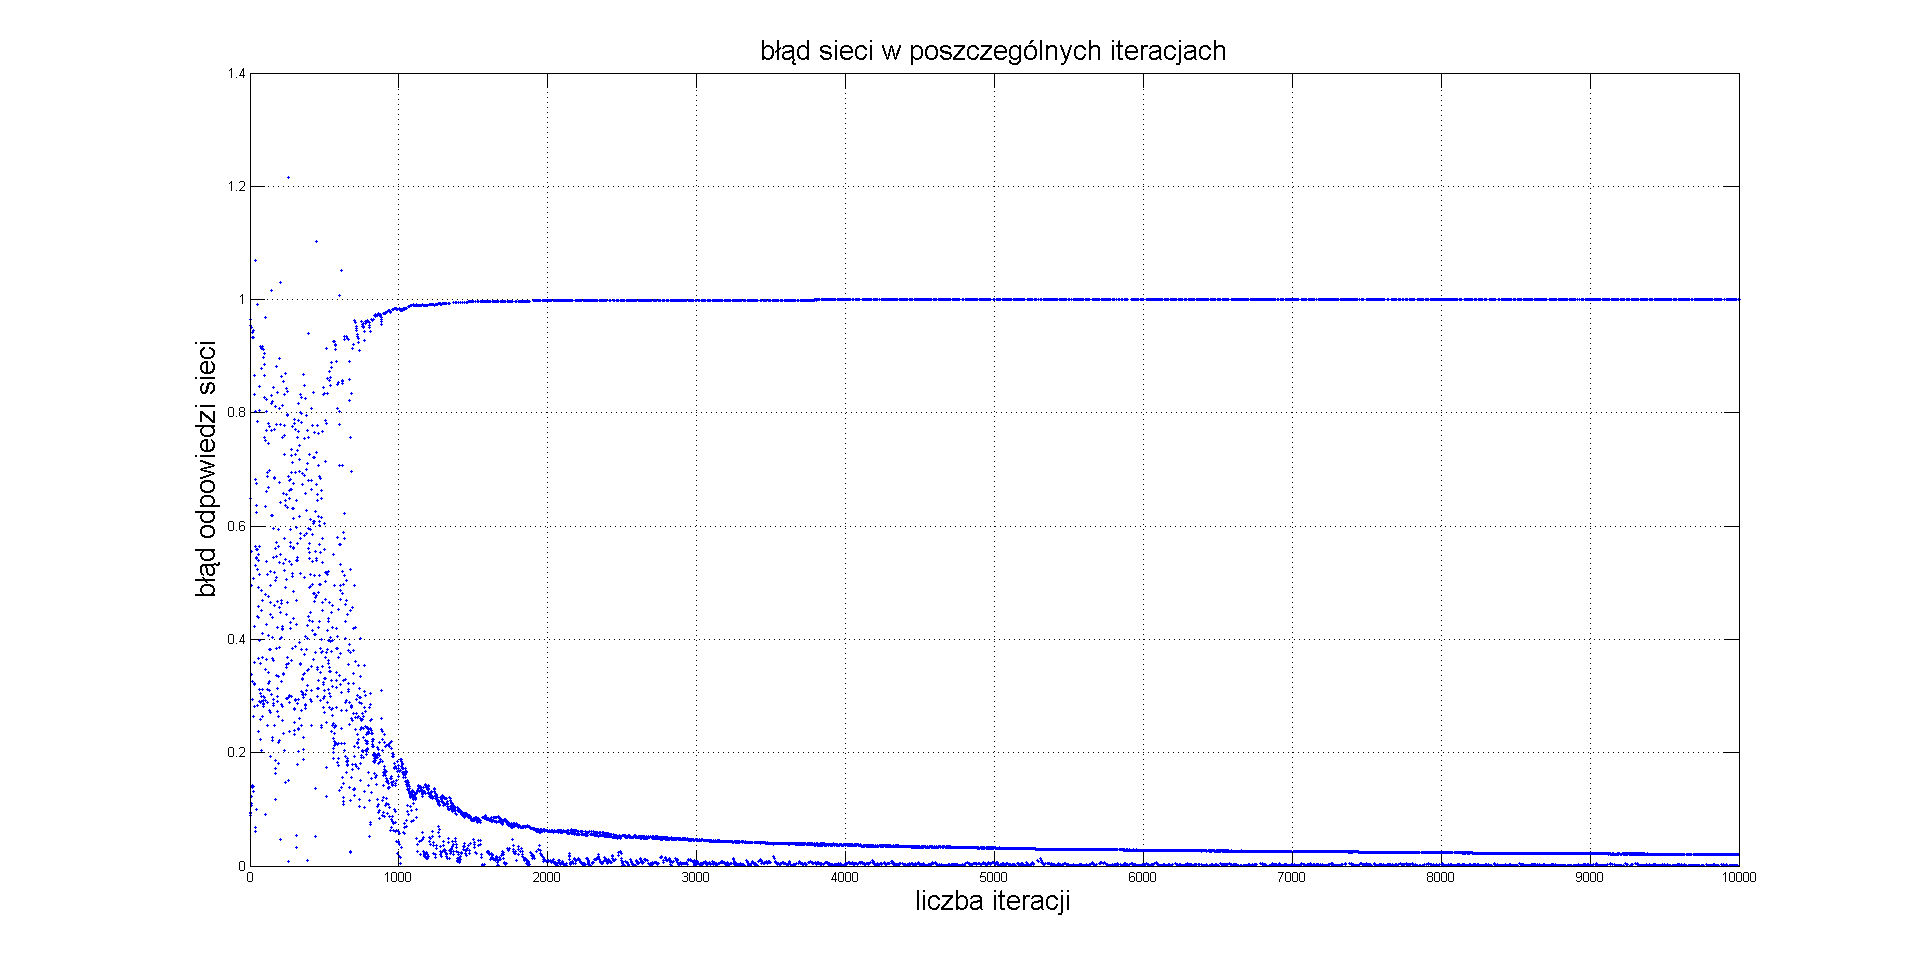
\includegraphics[width=1\linewidth]{./include/topologia_2_1}
\caption{Wykres błędu w kolejnych iteracjach dla sieci o topologii 2-1.}
\label{fig:neuro_2_1}
\end{figure}

\begin{table}
\centering

\label{tab:xor_output_2_1}
\begin{tabular}{|r|l|l|}
  \hline 
  Wejście 1 & Wejście 2 & Wyjście \\
  \hline 
  0 & 0 & 0 \\
  \hline
  0 & 1 & 1 \\
  \hline
  1 & 0 & 1 \\
  \hline
  1 & 1 & 0 \\
  \hline
\end{tabular}
\caption{Odpowiedzi sieci neuronowej o topologii 2-1.}
\end{table}

Na podstawie powyższego zestawienia: wykresu \ref{fig:neuro_2_1}, oraz tabeli \ref{tab:xor_output_2_1} można uznać, iż weryfikacja potwierdziła wcześniejszą tezę teoretyczną, która zakłada, iż sieć neuronowa nie posiadająca ukrytej warstwy nie jest w stanie rozwiązać zagadnień nieliczniowych. Jednocześnie potwierdza to, zgodność implementacji z teorią dotyczącą sieci neuronowych.

\begin{figure}[!htbp]
\centering
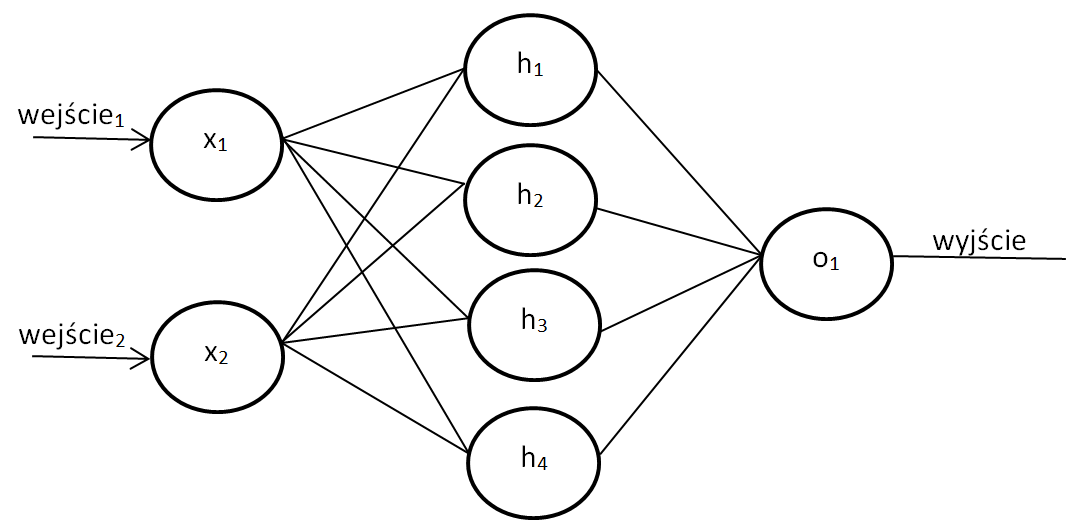
\includegraphics[width=0.7\linewidth]{./include/flow_2_4_1}
\caption{Przepływ informacji w topologii 2-4-1.}
\label{fig:flow_2_4_1}
\end{figure}

Następnie przeprowadzono test sieci w topologi przedstawionej na rysunku \ref{fig:neuro_2_4_1}.

W stosunku do poprzedniego testu, architektura sztucznej sieci neuronowej została rozbudowana o dodatkową warstwę ukrytą. Pozostałe cechy sieci takie jak inicjalizacja wag neuronów oraz funkcja aktywacji pozostały bez zmian.

\begin{figure}[!htbp]
\centering
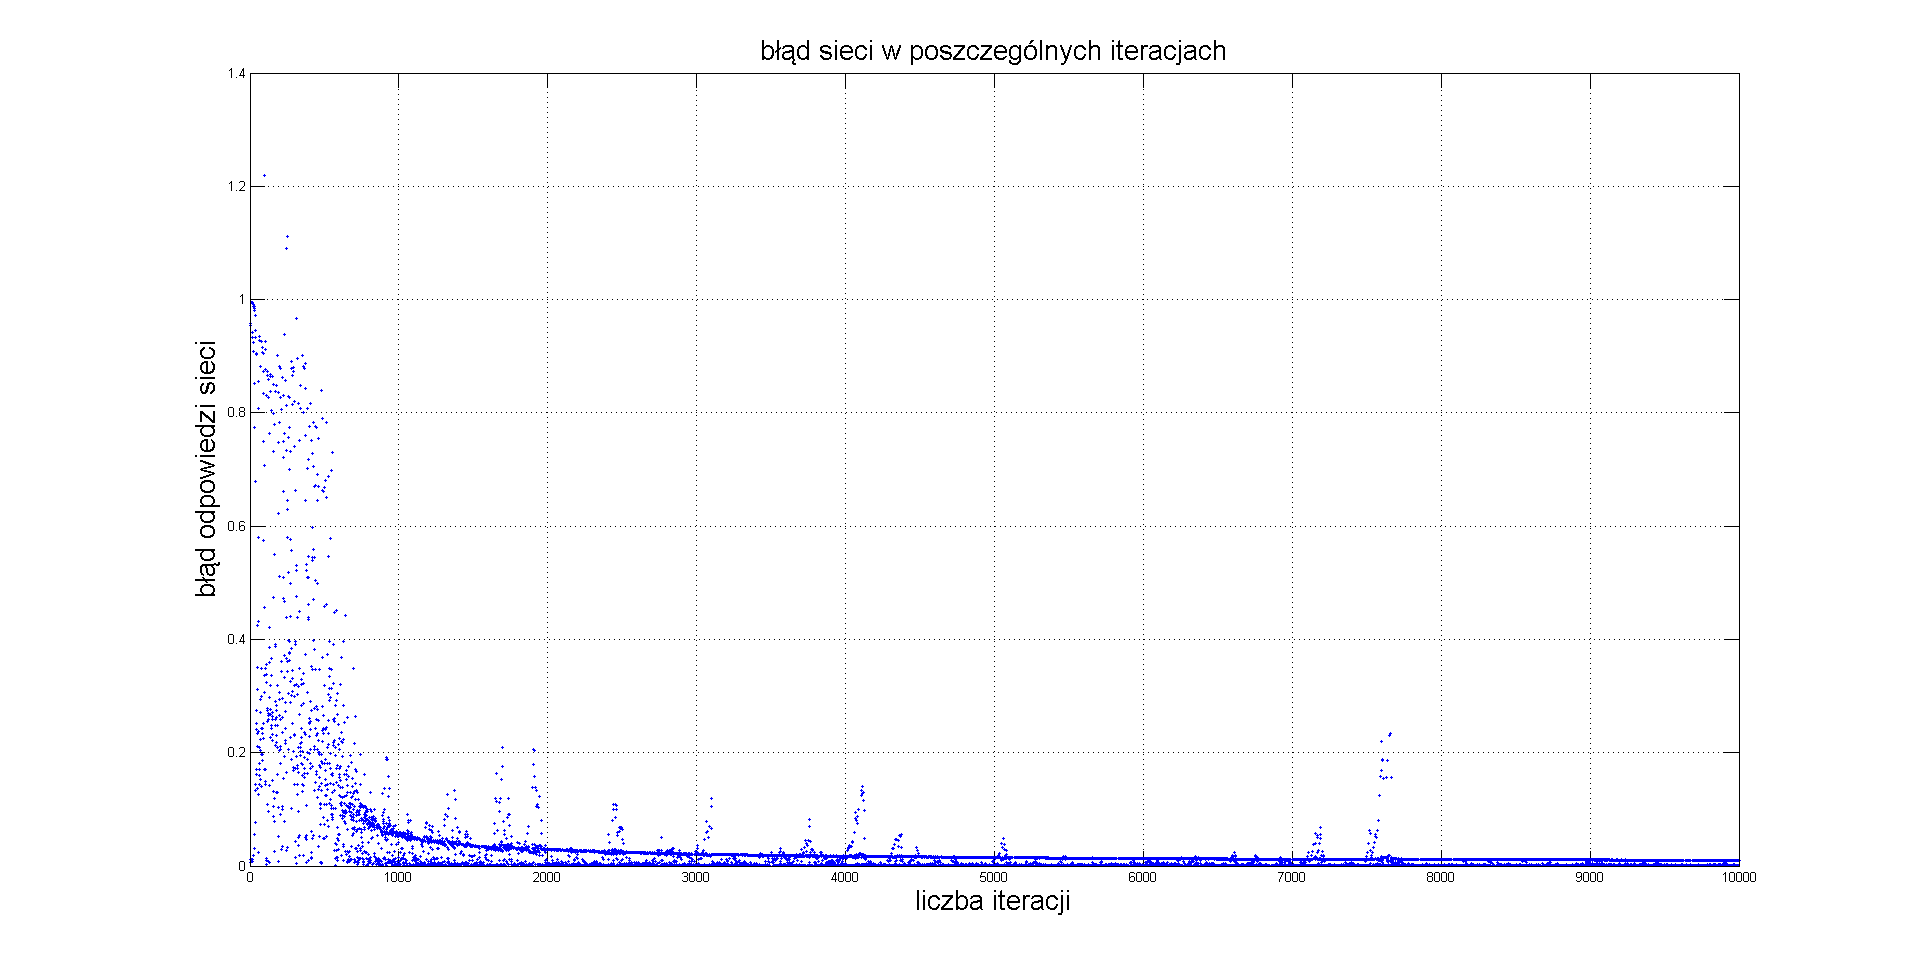
\includegraphics[width=1\linewidth]{./include/topologia_2_4_1}
\caption{Wykres błędu w kolejnych iteracjach dla sieci o topologii 2-4-1.}
\label{fig:neuro_2_4_1}
\end{figure}

%TODO wnioski do uczenia sieci

\begin{table}
\centering

\label{tab:xor_output_2_4_1}
\begin{tabular}{|r|l|l|}
  \hline 
  Wejście 1 & Wejście 2 & Wyjście \\
  \hline 
  0 & 0 & 0 \\
  \hline
  0 & 1 & 1 \\
  \hline
  1 & 0 & 1 \\
  \hline
  1 & 1 & 0 \\
  \hline
\end{tabular}
\caption{Odpowiedzi sieci neuronowej o topologii 2-4-1.}
\end{table}

\section{Testy działania algorytmu sterowania opartego na sztucznej sieci neuronowej}
